\documentclass[a4paper]{article}
\usepackage[margin=3.5cm]{geometry}
\usepackage{amsmath}
\usepackage{amssymb}
\usepackage[svgnames]{xcolor}
\usepackage{amsthm}
\usepackage{dsfont}
\usepackage{graphicx}
\usepackage{hyperref}
\usepackage{datetime}
\usepackage{outlines}
\usepackage{float}
\usepackage{booktabs}
\usepackage{enumitem}


\definecolor{fgcolor}{rgb}{0.345, 0.345, 0.345}
\newcommand{\hlnum}[1]{\textcolor[rgb]{0.686,0.059,0.569}{#1}}%
\newcommand{\hlstr}[1]{\textcolor[rgb]{0.192,0.494,0.8}{#1}}%
\newcommand{\hlcom}[1]{\textcolor[rgb]{0.678,0.584,0.686}{\textit{#1}}}%
\newcommand{\hlopt}[1]{\textcolor[rgb]{0,0,0}{#1}}%
\newcommand{\hlstd}[1]{\textcolor[rgb]{0.345,0.345,0.345}{#1}}%
\newcommand{\hlkwa}[1]{\textcolor[rgb]{0.161,0.373,0.58}{\textbf{#1}}}%
\newcommand{\hlkwb}[1]{\textcolor[rgb]{0.69,0.353,0.396}{#1}}%
\newcommand{\hlkwc}[1]{\textcolor[rgb]{0.333,0.667,0.333}{#1}}%
\newcommand{\hlkwd}[1]{\textcolor[rgb]{0.737,0.353,0.396}{\textbf{#1}}}%
\let\hlipl\hlkwb

\usepackage{framed}
\makeatletter
\newenvironment{kframe}{%
 \def\at@end@of@kframe{}%
 \ifinner\ifhmode%
  \def\at@end@of@kframe{\end{minipage}}%
  \begin{minipage}{\columnwidth}%
 \fi\fi%
 \def\FrameCommand##1{\hskip\@totalleftmargin \hskip-\fboxsep
 \colorbox{shadecolor}{##1}\hskip-\fboxsep
     % There is no \\@totalrightmargin, so:
     \hskip-\linewidth \hskip-\@totalleftmargin \hskip\columnwidth}%
 \MakeFramed {\advance\hsize-\width
   \@totalleftmargin\z@ \linewidth\hsize
   \@setminipage}}%
 {\par\unskip\endMakeFramed%
 \at@end@of@kframe}
\makeatother

\definecolor{shadecolor}{rgb}{.97, .97, .97}
\definecolor{messagecolor}{rgb}{0, 0, 0}
\definecolor{warningcolor}{rgb}{1, 0, 1}
\definecolor{errorcolor}{rgb}{1, 0, 0}
\newenvironment{knitrout}{}{} % an empty environment to be redefined in TeX


% code highlighting
\usepackage{minted}
\usepackage{xpatch}
\newminted[cminted]{python}{fontsize=\small}
\xpretocmd{\cminted}{\RecustomVerbatimEnvironment{Verbatim}{BVerbatim}{}}{}{}

% link coloring
%\hypersetup{
%    colorlinks,
%    linkcolor={red!80!black},
%    citecolor={green!60!black},
%    urlcolor={blue!80!black}
%}

% concatenation symbol (c.f. ++ in Haskell)
\newcommand\mdoubleplus{\mathbin{+\mkern-10mu+}}

% end of proof symbol
\newcommand{\newmarkedtheorem}[1]{%
  \newenvironment{#1}
    {\pushQED{\qed}\csname inner@#1\endcsname}
    {\popQED\csname endinner@#1\endcsname}%
  \newtheorem{inner@#1}%
}

\theoremstyle{definition}
%\newtheorem{eg}{Example}[section]
\newmarkedtheorem{eg}{Example}[section]
\newtheorem{observation}{Observation}[section]
\newtheorem{define}{Definition}[section]
\theoremstyle{plain}
\newtheorem{proposition}{Proposition}
\newtheorem{lemma}{Lemma}
\newtheorem{corollary}{Corollary}
\newtheorem{theorem}{Theorem}[section]
\newtheorem{assump}{Assumption}[section]
\newtheorem{remark}{Remark}[section]

\newdateformat{monthyeardate}{\monthname[\THEMONTH] \THEYEAR}

\author{Jeroen van Riel}
\date{\monthyeardate\today}
\title{Trajectory Optimization of Autonomous Vehicles in Networks of Intersections}

\begin{document}

\maketitle

\tableofcontents

\section{Trajectories in tandem of two intersections}

\begin{figure}
  \centering
  \makebox[\textwidth][c]{% wider than textwidth
    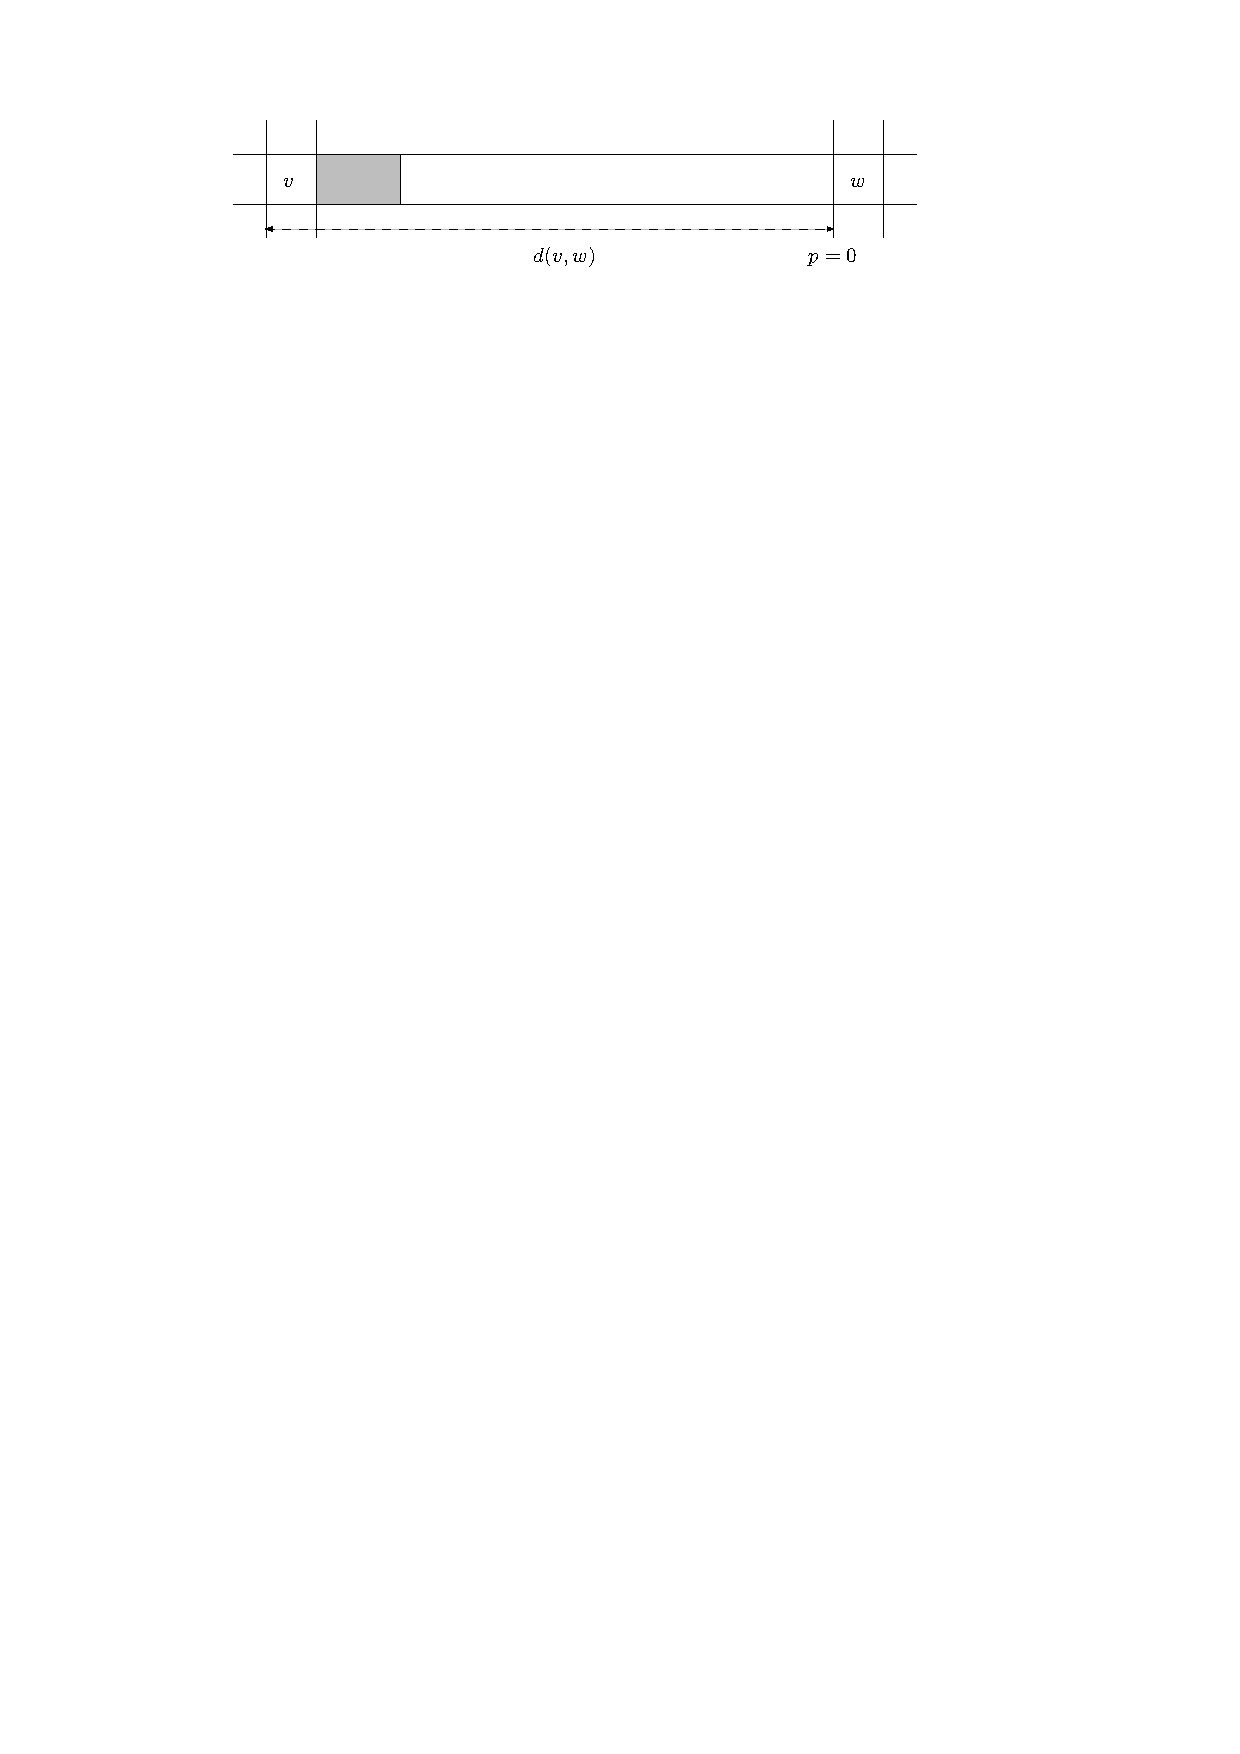
\includegraphics[width=1.0\textwidth]{figures/motion/tandem}
  }
  \caption{Tandem of two intersections $v$ and $w$ with lane of length $d(v,w)$.
    The grey rectangle represents some vehicle that just left intersection $v$.
    We will assume that a vehicle has maximum speed as long as it occupies an
    intersection, so it is only allowed to decelerate once it passes this
    position.}
  \label{fig:tandem}
\end{figure}

When considering multiple vehicle driving between intersection, we can no longer
ignore the issue of road capacity, because the fact that only a limited number
of vehicles can drive or wait at the same time on a lane between intersections
may cause network-wide effects.
%
The capacity of lanes between intersections
is intimately related to the trajectories of vehicles, which we first want to
understand better. We have been using an optimal control formulation with the
objective that keeps the vehicles as close as possible to the next intersection
at all times (\texttt{MotionSynthesize}). This problem can be solved using
direct transcription, which works well enough if we just want to simulate the
behavior of the system. However, we believe that it is possible to explicitly
formulate the optimal controller. We will explain how to compute trajectories
corresponding to those obtained by direct transcription, but without using time
discretization.

Before we turn to the general case of networks of intersection, we will first
investigate the trajectories of vehicles in a tandem of two intersections as
depicted in Figure~\ref{fig:tandem}. Let $v$ denote the left intersection and
$w$ the right intersection and assume that vehicles drive from left to right.
% We will sometimes refer to intersection $w$ as the downstream intersection.
Furthermore, we will call the road segment strictly between both intersection
areas the \textit{lane}. To facilitate the following discussion, we will use $p$
to denote the position of a vehicle to distinguish it from the state
$x = (p, v)$, which also includes the velocity, and we fix position $p=0$ at the
stop-line of intersection $w$. Let the length and width of a vehicle $i$ be
denoted by $L_{i}$ and $W_{i}$, respectively. We measure the position of a
vehicle at the front bumper.
%
We will make the following assumption, that allow us to easily derive explicit
expressions of these trajectories.

\begin{assump}
  \label{assump:same_geometry}
  All vehicles have the same length $L_{i} = L$ and width $W_{i} = W$. Lanes
  are exactly $W$ units wide and are axis-aligned, such that intersection are
  squares.
\end{assump}

\begin{assump}
  \label{assump:full_speed}
  Vehicles must drive at full speed when entering an intersection and keep
  driving at full speed as long as they occupy an intersection.
\end{assump}

Now assume that some vehicle is scheduled to exit $v$ at time $t_{0}$ and to
enter $w$ at some time $t_{f}$. Let $p_{0} = -d(v,w) + W$ denote the position of
the vehicle when it starts to exit $v$. Let $y(t)$ denote the trajectory of the
vehicle that drives in front of the current one, assuming it exists. In order to
keep the vehicle as close to $w$ as possible at every time, while respecting
the double integrator vehicle dynamics $\dot{p} = v, \, \ddot{p} = u$, we can
generate a trajectory by solving the optimal control problem
\begin{equation}
  \label{eq:optimal_control}
  \begin{aligned}
  \max_{u}    \quad & \int_{t_{0}}^{t_{f}} p(t) dt \\
  \begin{alignedat}{2}\text{s.t.}\\ {}\end{alignedat} \quad &\begin{alignedat}{2}
                     0 \leq \; &v(t) \leq v_{\max} , \\
                     {-a_{\max}} \leq \; &u(t) \leq a_{\max} , \\
                    y(t) \leq \; & p(t) , \\
                    \end{alignedat} \\
                    &\begin{alignedat}[t]{2}
                    & p(t_{0}) = p_{0} , &&  p(t_{f}) = 0 , \\
                    & v(t_{0}) = v_{\max} , \;\; && v(t_{f}) = v_{\max} .
                    \end{alignedat}
  \end{aligned}
\end{equation}
%
This problem can be solved by using a direct transcription method. After
observing some example solutions, we believe that the optimal control should
switch between no acceleration and either full acceleration or full
deceleration, i.e., we have a control function $u(t) := \ddot{x}(t)$ satisfies
$u(t) \in \{-a_{\max}, 0, a_{\max}\}$ and some sequence of alternating
deceleration and acceleration periods, represented by some sequence of disjoint
intervals
\begin{align*}
  (D_{0}, A_{1}, D_{1}, \dots, A_{n-1}, D_{n-1}, A_{n}) ,
\end{align*}
so that the optimal controller is given by
\begin{align*}
  u(t) = \begin{cases}
           {-a_{\max}} &\text{ if } t \in D_{k} \text{ for some } k , \\
           \phantom{-} a_{\max}   &\text{ if } t \in A_{k} \text{ for some } k , \\
           \phantom{-} \;\, 0 &\text{ otherwise. }
         \end{cases}
\end{align*}

\subsection{Single vehicle}

We can proof the above hypothesis and provide explicit expressions for $D_{k}$
and $A_{k}$ of the optimal trajectory whenever the safe following constraint
$y(t) \leq p(t)$ is never active and can essentially be ignored, either because
there is no vehicle ahead or it is sufficiently far away.
%
The proof uses a variant of the Pontryagin Maximum Principle, specifically
tailored to problems with state
constraints~\cite{hartlSurveyMaximumPrinciples1995}.

\newpage

\begin{figure}
  \centering
  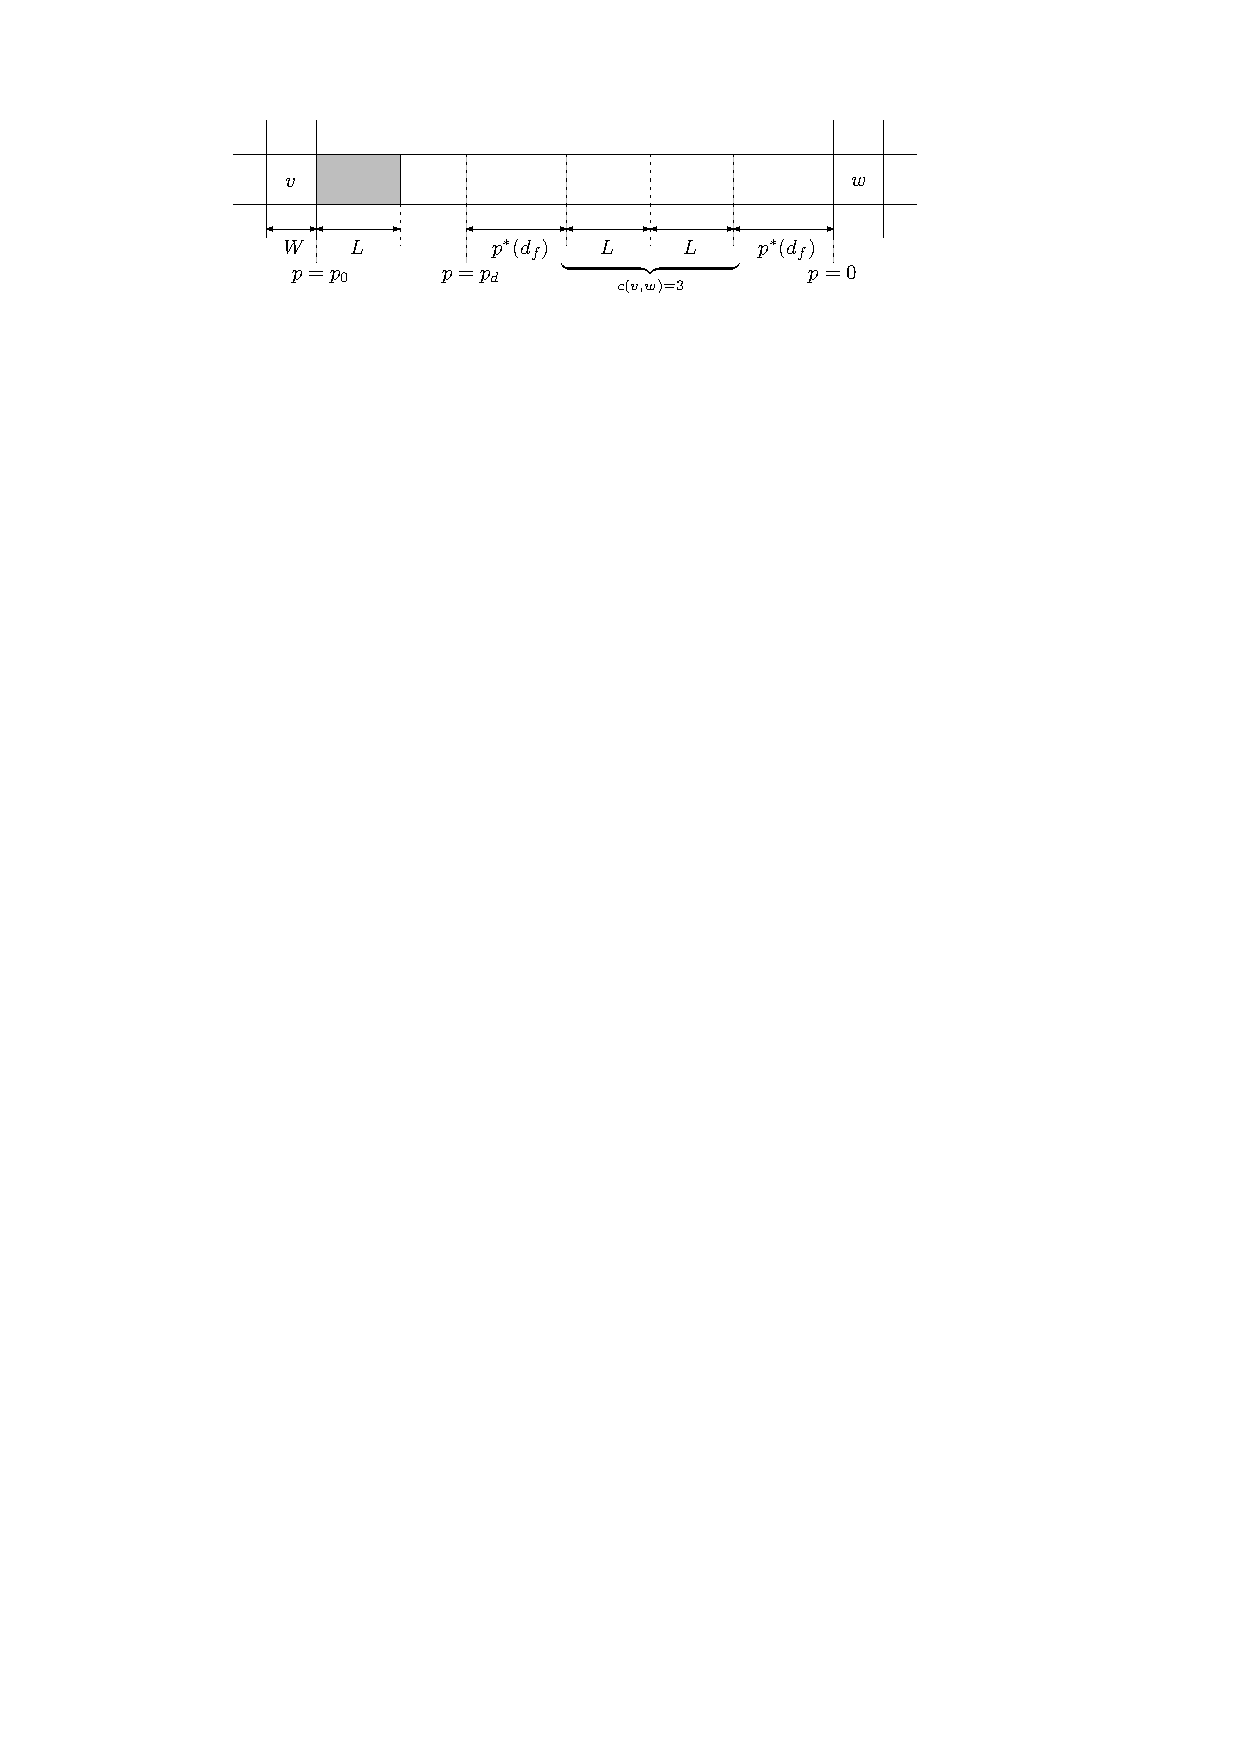
\includegraphics[width=0.99\textwidth]{figures/motion/tandem_annotated}
  \caption{Tandem of intersections with distances used in the determination of
    the lane capacity and the waiting positions.}
  \label{fig:tandem_annotated}
\end{figure}

\subsection{Multiple vehicles}

By observing optimal trajectories generated using direct transcription, we
observe that there is a lot of structure in how the trajectory of a vehicle
influences the trajectories of later vehicles. In this section, we provide a
direct way to explicitly calculate trajectories, without proving that these
trajectories are always feasible and optimal. Instead, we verify correctness of
our method numerically by comparing the output to direct transcription for
various system parameters and crossing times.

We start by investigating the limit on the number of vehicles that can occupy
the lane at the same time. Imagine that vehicles enter the lane until it is full
and then only after all vehicles have come to a full stop, they start to leave
the lane by crossing $w$.
%
Without any additional constraints, it follows from the vehicle dynamics that
the time it takes to fully accelerate from rest to maximum velocity is given by
$d_{f} = v_{\max} / a_{\max}$ and with corresponding trajectory
\begin{align*}
  p^{*}(t) = a_{\max} t^{2} / 2 \quad \text{ for } 0 \leq t \leq d_{f} .
\end{align*}
Because we assume that maximum
deceleration is also $a_{\max}$, it also takes $d_{f}$ time to fully decelerate
from maximum velocity to rest.
%
Suppose that we want to design the tandem network such that at least $c(v,w)$
vehicles can enter and decelerate to some waiting position, from which it is
also possible to accelerate again to full speed before crossing $w$.
%
Vehicles are required to drive at full speed as long as they occupy
any intersection. Therefore, a vehicle crossing $v$ can only start decelerating
after $p(t) \geq W + L$, so the earliest position where a vehicle can come to a
stop is $p = W + L + p^{*}(d_{f})$.
%
Because vehicles need to gain maximum speed before reaching $w$,
the position closest to $w$ where a vehicle can wait is $- p^{*}(d_{f})$.
%
Hence, in order to accomodate for $c(v,w)$ waiting vehicles, the length of the
lane must satisfy
\begin{align*}
  d(v, w) \geq W + L + 2p^{*}(d_{f}) + (c(v,w) - 1) L ,
\end{align*}
as illustrated in Figure~\ref{fig:tandem_annotated}.
%
Conversely, given the lane length $d(v,w)$, the corresponding lane capacity is
given by
\begin{align*}
  c(v, w) = \texttt{floor}\left( \frac{d(v,w) - W - 2 p^{*}(d_{f})}{L} \right) ,
\end{align*}
where $\texttt{floor}(x)$ denotes the largest integer smaller than or equal to
$x$.

% emphasize fixed locations
It turns out that the fixed locations where vehicles wait in the above scenario
are helpful in describing the optimal trajectories, even when vehicles never
fully stop. We will denote these fixed \textit{waiting positions} as
\begin{align*}
  p_{k} = - p^{*}(d_{f}) - (c(v,w) - k) L,
\end{align*}
for $k = 1, \dots, c(v,w)$.
%
Furthermore, let $p_{d} = p_{1} - p^{*}(d_{f})$ denote the position from
which vehicles must decelerate in order to stop at the earliest waiting position
$p_{1}$, which is the farthest from the destination intersection.
%
Now consider a vehicle that moves from $p_{k}$ to the next waiting position
$p_{k+1}$, so it moves exactly distance $L$. We consider such a start-stop
movement, without considering any safe following constraints. By symmetry of the
control constraints, the vehicle moves the same distance during both
acceleration and deceleration. Furthermore, the vehicle needs to be at rest at
the start and end of such trajectory. Hence, it is clear that it takes the same
amount of time $d_{s}$ to accelerate and decelerate. We assume that
$d_{s} < d_{f}$, which ensures that $v_{\max}$ is never reached during the
start-stop movement, which is illustrated in Figure~\ref{fig:start-stop}. In this case, it is
clear that we must have $L = 2 p^{*}(d_{s})$, from which we derive that
$d_{s} = \sqrt{L / a_{\max}}$.

\subsubsection{Ad-hoc approach}
We will now present a method to calculate the trajectory of a vehicle based on
its crossing times at $v$ and $w$ and the trajectory of the vehicle ahead of it.
We start from a sequence of deceleration and acceleration intervals that are
possibly overlapping and then merge them in pairs from left to right until they
become disjoint.
%
Specifically, let
\begin{align*}
  t_{d} := t_{0} + \frac{d(v,w) - W - p_{d}}{v_{\max}}
\end{align*}
be the start of the initial deceleration interval
$D_{0} := [t_{d}, t_{d} + d_{f}]$, which is exactly the moment the vehicle needs
to start decelerating in order to stop at the first waiting position $p_{1}$, so
at time $t_{d}$ the vehicle is at position $p_{d}$. Similarly, let
$t_{a} = t_{f} - d_{f}$ be the start of the final acceleration interval
$A_{f} := [t_{a}, t_{a} + d_{f}]$. Now for every $k = 1, \dots, c(v,w) - 1$, we
consider a pair of start-stop intervals
$S_{k} := (A_{k}, D_{k}) = ([t_{k}, t_{k} + d_{s}], [t_{k} + d_{s}, t_{k} + 2 d_{s}])$
at some starting time $t_{k}$, moving the vehicle from $p_{k}$ to $p_{k+1}$. We
first show how to merge these intervals such that a sequence of disjoint
intervals is obtained. Afterwards, we show how times $t_{k}$ follow from the
trajectory of the vehicle ahead.

% show how to merge, assuming $S_{n}$ are disjoint
First, we show how to merge $D_{0}$ and $S_{1}$.
% case 1: separate
When we have $t_{d} + d_{f} \leq t_{1}$, it is clear that both parts are already
completely disjoint, so we do not have to do anything further.
% case 2: merging
As $t_{d}$ and $t_{1}$ get closer than $d_{f}$, we need to start merging $D_{0}$
and $A_{1}$ as we will show. In this case, we observe that $D_{0}$ gets shorter
at the end by some $\epsilon$ and the acceleration part of $S_{1}$ gets shorter at the
beginning, also by the same amount $\epsilon$, because the velocities must match. More
precisely, we construct two new consecutive intervals
\begin{align*}
  D_{0}' &= [t_{1} + 2 \epsilon - d_{f}, \; t_{1} + \epsilon] , \\
  A_{1}' &= [t_{1} + \epsilon,   \; t_{1} + d_{s}],  \\
  D_{1}  &= [t_{1} + d_{s},      \; t_{1} + 2 d_{s}] .
\end{align*}
%
We now determine $\epsilon$ as a function of $t_{1} - t_{d}$.
%
Because $D_{0}'$ and $A_{1}'$ are both $\epsilon$ shorter, the total distance
that is traversed is now $2 p^{*}(\epsilon)$ shorter. This means that the start
of $D_{0}'$ should be $2 p^{*}(\epsilon) / v_{\max}$ later than $t_{d}$, which
gives equation
\begin{align*}
  t_{d} + \frac{2 p^{*}(\epsilon)}{v_{\max}}  = t_{1} + 2\epsilon - d_{f} ,
\end{align*}
which is quadratic in $\epsilon$. Because we must have $\epsilon < d_{f}$, we need the
smallest solution
\begin{align*}
  \epsilon = d_{f} - \sqrt{d_{f} (t_{1} - t_{d})} .
\end{align*}
% case 3: merged
When we keep increasing $t_{d}$ while keeping $t_{1}$ fixed, we observe that
eventually part $A_{1}$ will completely disappear and $D_{0}$ and $D_{1}$ will
become a single interval, which is easily seen to happen when $\epsilon \geq d_{s}$.
Equivalently, this happens when $t_{d}$ is such that
$t_{d} \geq t_{1} - d_{f} + 2 d_{s} - 2p^{*}(d_{s}) / v_{\max}$.

% merge start-stops (AD-AD)
We now show how two start-stop parts have to be merged if they overlap. Consider
two start-stop parts $A_{k},D_{k}$ and $A_{k+1},D_{k+1}$ and suppose that
$t_{k} + 2 d_{s} < t_{k+1}$ such that both parts have to be merged. The parts
$D_{k}$ and $A_{k+1}$ merge by removing $\epsilon$ on both sides, similarly as
above. However, this causes the $D_{k},A_{k+1},D_{k+1}$ parts to shift up.
Therefore, $A_{k}$ and $D_{k}$ each need to be lengthened at the side where they
meet by some $\delta$ to match this.
%
Hence, it turns out we have to use the intervals
\begin{align*}
  A_{k}' &= [t_{k}, t_{k} + d_{s} + \delta] , \\
  D_{k}' &= [t_{k} + d_{s} + \delta, t_{k+1} + \epsilon] , \\
  A_{k+1}' &= [t_{k+1} + \epsilon, t_{k+1} + d_{s} ] , \\
  D_{k+1} &= [t_{k+1}, t_{k+1} + d_{s}] .
\end{align*}
%
We have that $\epsilon$ and $\delta$ need to satisfy
\begin{align*}
  \begin{cases}
  2\delta + 2\epsilon = t_{k+1} - t_{k} , \\
  2p^{*}(d_{s}+\delta) - 2p^{*}(d_{s} - \epsilon) = L .
  \end{cases}
\end{align*}
Solving this system of equations yields
\begin{align*}
  \delta &= \frac{L / a_{\max}}{t_{k+1} - t_{k}} - d_{s} + \frac{t_{k+1} - t_{k}}{4} , \\
  \epsilon &= (t_{k+1} - t_{k}) / 2 - \delta .
\end{align*}
%

Finally, we consider the merge with the final acceleration bang.

Note that the above types of merging are enough to process the whole sequence of
bangs, because when the first merge of $D_{0}$ and $A_{1},D_{1}$ results in a
single $D_{1}'$ and there is a next $A_{2},D_{2}$, we are again in the first
situation.

% show how $S_{n}$ follow from predecessor
We now show how $t_{k}$ follow from the trajectory of the preceding vehicle.

\begin{figure}
  \centering
  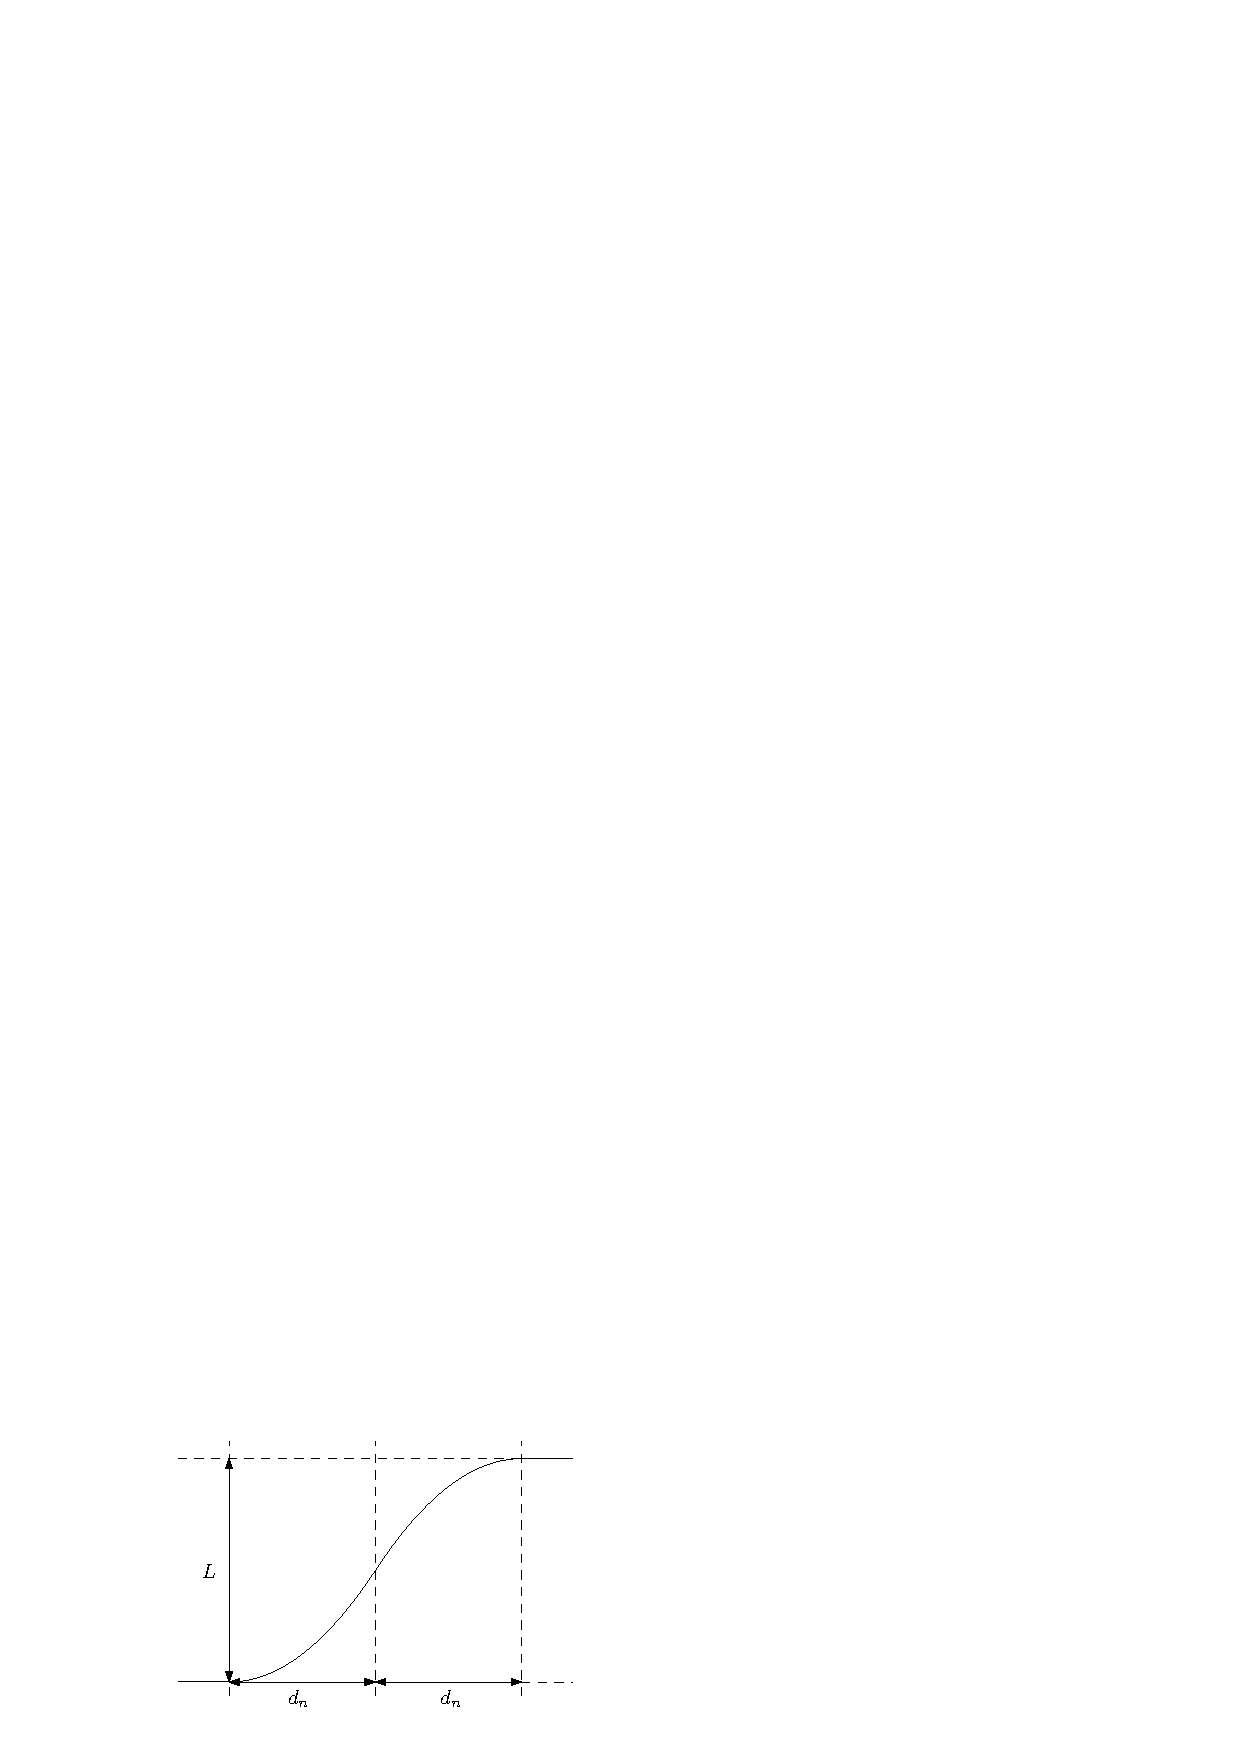
\includegraphics[scale=1.0]{figures/motion/start_stop_trajectory}
  \caption{Shape of some start-stop trajectory of a single isolate vehicle
    moving forward from some current waiting position $p_{k}$ to the next
    $p_{k+1}$.}
  \label{fig:start-stop}
\end{figure}

\begin{figure}
  \centering
  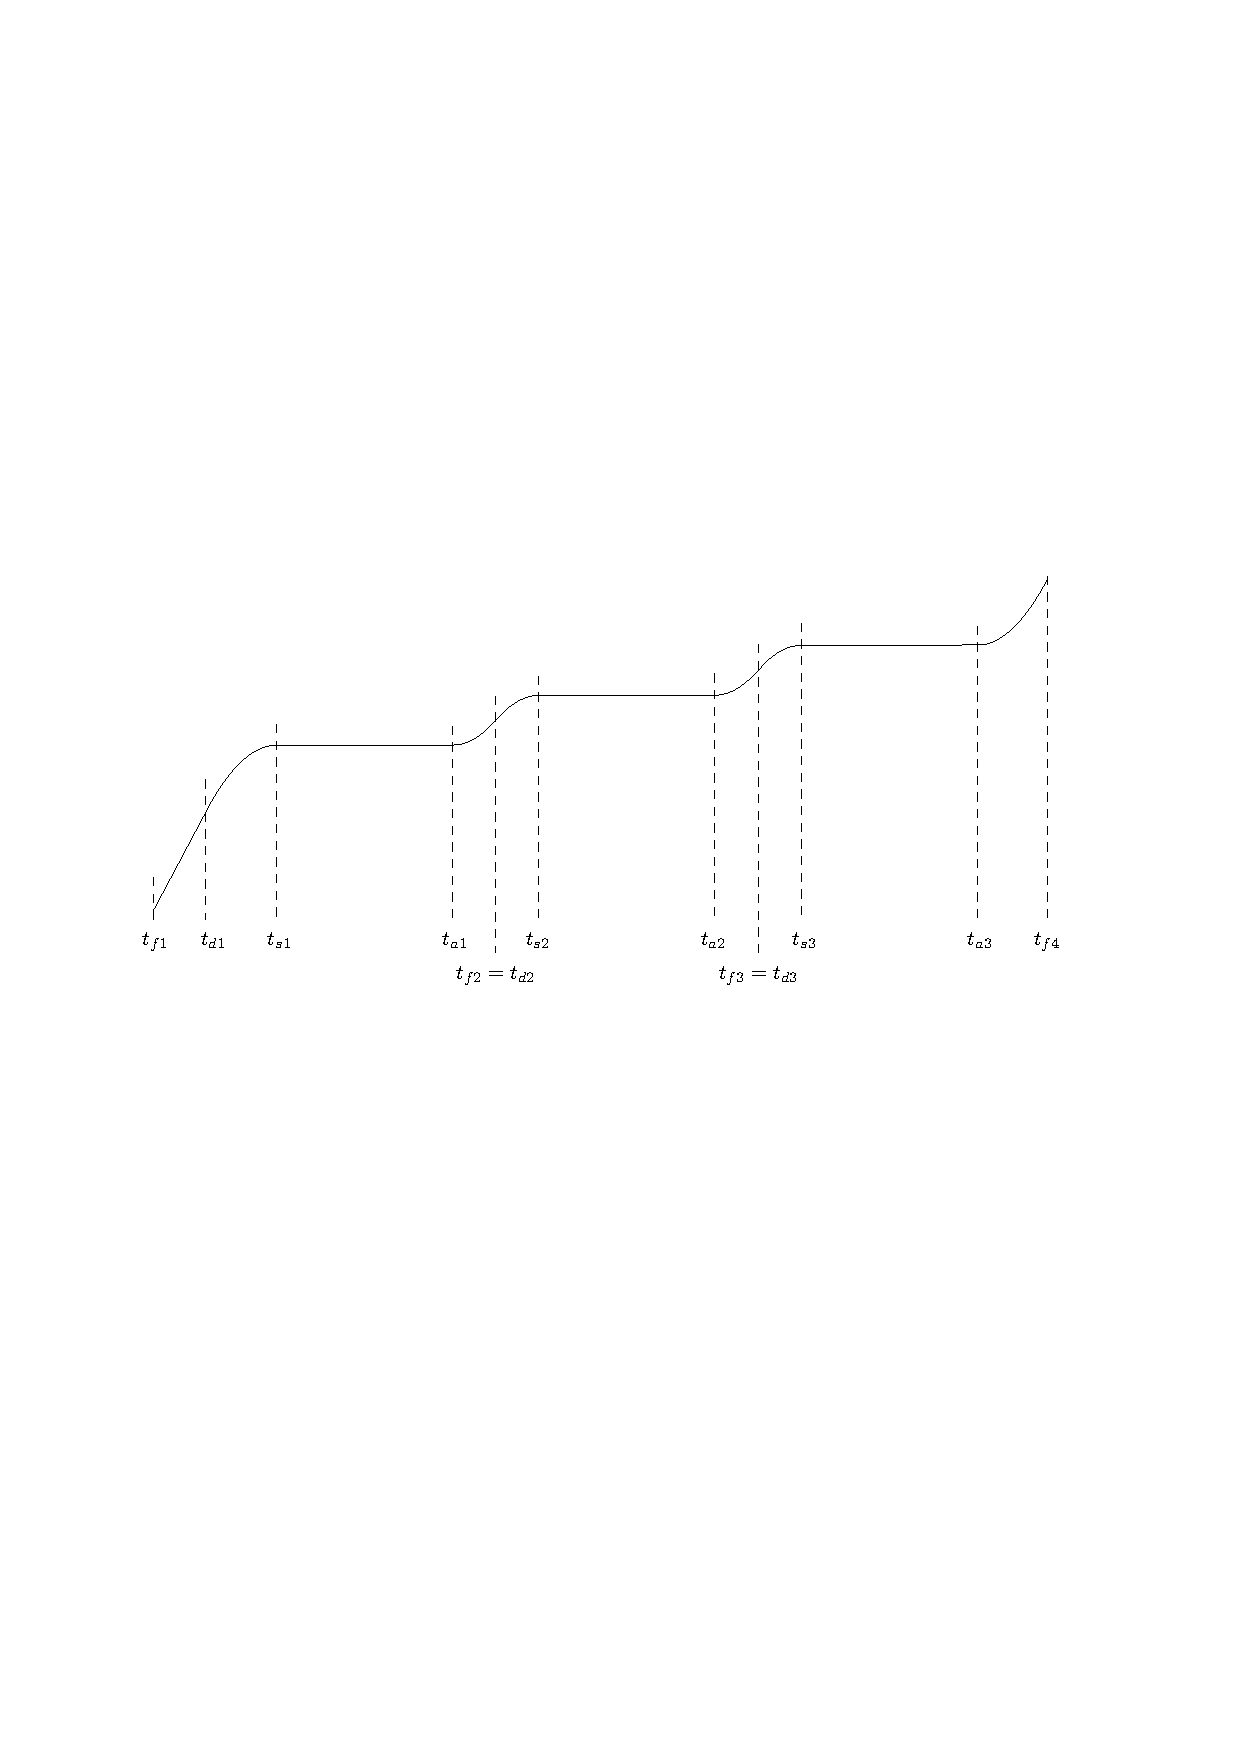
\includegraphics[width=0.8\textwidth]{figures/motion/tandem_trajectory}
  \caption{Sketch of vehicle trajectory in tandem with all the full start-stop
    parts unmerged.}
  \label{fig:tandem_trajectory}
\end{figure}

% \begin{figure}
%   \centering
%   \includegraphics[width=0.99\textwidth]{figures/motion/merge}
%   \caption{Sketch how the initial deceleration merges with the first start-stop phase.}
%   \label{fig:merge}
% \end{figure}

\subsubsection{Schedule time approach}

\newpage
\section{Trajectories in networks}

\begin{figure}
  \centering
  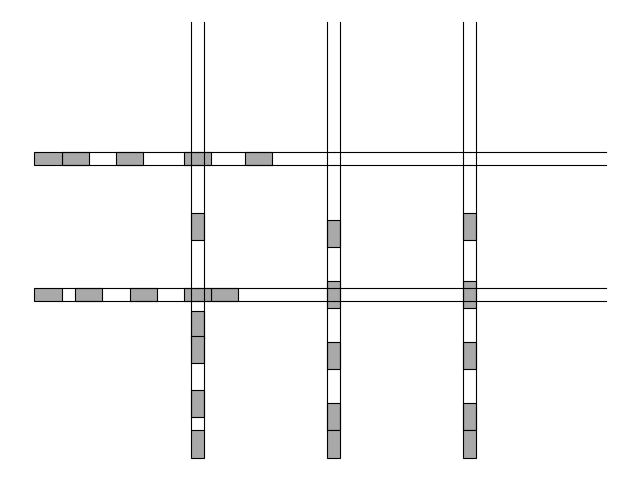
\includegraphics[width=0.55\textwidth]{figures/state_example.png}
  \caption{Illustration of some grid-like network of intersections with vehicles
    drawn as grey rectangles. There are five vehicle routes: two from east to
    west and three from south to north. Turning at intersections is not
    allowed.}\label{fig:network_illustration}
\end{figure}

We now extend the single intersection model to a network of intersections
without turning routes, illustrated in Figure~\ref{fig:network_illustration}.
% network definition
We define a directed graph $(V,E)$ with nodes $V$ and arcs $E$, representing the
possible paths that vehicles can follow. Nodes of in-degree at least two are
called \textit{intersections}. Nodes with only outgoing arcs are
\textit{entrypoints} and nodes with only incoming arcs are \textit{exitpoints}.
%
Let $d(v, w)$ denote the distance between nodes $v$ and $w$.
%
For each route index $r \in \mathcal{R}$, we let
\begin{align*}
  \bar{V}_{r} = (v_{r}(0), v_{r}(1), \dots, v_{r}(m_{r}), v_{r}(m_{r+1}))
\end{align*}
be the path that vehicles $i \in \mathcal{N}_{r}$ follow through the network. We
require that the first node $v_{r}(0)$ is an entrypoint and that the last node
$v_{r}(m_{r+1})$ is an exitpoint and we write
\begin{align*}
  V_{r} = \bar{V}_{r} \setminus \{ v_{r}(0), \, v_{r}(m_{r+1}) \}
\end{align*}
to denote the path restricted to intersections. We say that some $(v, w) \in E$
is on path $V_{r}$ whenever $v$ and $w$ are two consecutive nodes on the path
and we write $E_{r}$ to denote the set of all these edges. We require that
routes can only overlap at nodes by making the following assumption.

\begin{assump}\label{assump:disjoint_routes}
  Every arc $(v,w) \in E$ is part of at most one route $V_{r}$.
\end{assump}

We start by considering networks in which all roads are axis-aligned such that
intersections always involve perpendicular lanes and where routes are such that
no turning is required. For each $v \in V_{r}$ define the conflict zone
$\mathcal{E}_{r}(v) = (b_{r}(v), e_{r}(v))$ and consider the union
\begin{align*}
  \mathcal{E}_{r} = \bigcup_{v \in V_{r}} \mathcal{E}_{r}(v)
\end{align*}
corresponding to the positions of vehicles $i \in \mathcal{N}_{r}$ for which it
occupies an intersection on its path $V_{r}$.
%
By reading $\mathcal{E}_{i} \equiv \mathcal{E}_{r}$ for $r(i) = r$, the single
intersection problem naturally extends to the network case. Like before, the
resulting problem can be numerically solved by a direct transcription method.

\subsection{General decomposition}
The general two-stage decomposition for the single intersection extends rather
naturally to the present model. Let for each pair $(i,v)$ of some vehicle
$i \in \mathcal{N}$ and an intersection $v \in V_{r(i)}$ along its route, let
\begin{align*}
\inf \{ t: x_{i}(t) \in \mathcal{E}_{r}(v) \} \;\; \text{ and } \; \sup \{ t: x_{i}(t) \in \mathcal{E}_{r}(v) \}
\end{align*}
be the crossing time and exit time, which we denote by $y(i,v)$ and
$y(i,v) + \sigma(i, v)$, respectively.
%
Instead of a single set of conflicts, we now define for each intersection
$v \in V$ in the network the set of conflict pairs
\begin{align*}
\mathcal{D}^{v} = \{ \{i,j\} \subset \mathcal{N} : r(i) \neq r(j), v \in V_{r(i)} \cap V_{r(j)} \} .
\end{align*}
Now the two-stage approach is to solve
\begin{align*}
  \min_{y,\sigma} \;\; & \sum_{r \in \mathcal{R}} F(y_{r}, \sigma_{r}) \\
  \text{ s.t. } & y(i,v) + \sigma(i,v) \leq y(j,v) \text{ or }  \\
                & y(j,v) + \sigma(j,v) \leq y(i,v) , & \text{ for all } \{i,j\} \in \mathcal{D}^{v} \text{ and } v \in V, \\
  & (y_{r}, \sigma_{r}) \in \mathcal{S}_{r} , \quad & \text{ for all } r \in \mathcal{R} ,
\end{align*}
%
where $F(y_{r}, \sigma_{r})$ and $\mathcal{S}_{r}$ are the value function and
set of feasible parameters, respectively, of the parametric trajectory
optimization problems
%
\begin{align*}
  F(y_{r}, \sigma_{r}) = \min_{x_{r}} & \; \sum_{r \in \mathcal{R}} J(x_{i}) \\
  \text{ s.t. } & x_{i}(t) \in D_{i}(s_{i,0}) , \quad & \text{ for } i \in \mathcal{N}_{r} , \\
  & x_{i}(y(i,v)) = b_{r}(v) , \quad & \text{ for } v \in V_{r} , i \in \mathcal{N}_{r} , \\
  & x_{i}(y(i,v) + \sigma(i,v)) = e_{r}(v) , \quad & \text{ for } v \in V_{r} , i \in \mathcal{N}_{r} , \\
  & x_{i}(t) - x_{j}(t) \geq L , \quad & \text{ for } (i, j) \in \mathcal{C} \cap \mathcal{N}_{r} ,
\end{align*}
where we again use subscript $r$ to group variables according to their associated route.


\subsection{Decomposition for delay objective}

Suppose we use use the crossing at the last intersection as performance measure, by defining the
objective function as
\begin{align*}
  J(x_{i}) = \inf \{ t: x_{i}(t) \in \mathcal{E}_{r}(v_{r}(m_{r}))\} .
\end{align*}
%
We show how to reduce the resulting problem to a scheduling problem, like we did
in the single intersection case.
%
It is not clear whether vehicles will always cross intersections at full speed,
but we will simply require vehicles to do so from here on.
Furthermore, we will again assume that all vehicles share the same geometry.
Hence, the
occupation time $\sigma \equiv \sigma(i,v)$ is the same for all vehicles and
intersections. For this reason, we will write the shorthand $y_{r} \in \mathcal{S}_{r}$,
because $\sigma_{r}$ is no longer a free variable.

%
As a consequence of Assumption~\ref{assump:same_geometry} and Assumption~\ref{assump:full_speed},
each lower-level trajectory optimization problem for a given route
$r \in \mathcal{R}$ decomposes into a sequence of problems, each corresponding to
two consecutive intersection along $V_{r}$.
%
This means that $y_{r} \in \mathcal{S}_{r}$ is equivalent to
$y_{(v,w)} \in \mathcal{S}_{(v,w)}$ for each $(v,w) \in E_{r}$, where
$y_{(v,w)}$ denotes the vector of all variables $y(i, v)$ and $y(i, w)$ for all
$i \in \mathcal{N}_{r}$ and $\mathcal{S}_{(v,w)}$ denotes the set of values of $y_{(v,w)}$ for which a feasible trajectory part can be found.
%
Hence, we will now focus on a tandem of two intersections and investigate the
trajectories of vehicles in this with the goal of stating sufficient conditions
for $y_{(v,w)} \in \mathcal{S}_{(v,w)}$.

\subsection{Crossing time scheduling}

% job-shop disjunctive graph
Introduce general job-shop problem and disjunctive graph.
% define travel constraints
Introduce travel constraints and explain corresponding new type of arc in disjunctive graph.
% define buffer constraints
Introduce buffer constraints and corresponding new arc in disjunctive graph.

\subsection{Branch-and-bound}
Formulate MILP problem and investigate how the solving time scales with network
size in terms of number of intersections and number of vehicles in the network.
Doe the single intersection cutting planes still hold? Are there any obvious
cutting planes?

\section{Constructive heuristic}

Like for problems with a single intersection, we want to investigate possible
constructive heuristics
%
In this case, the step-by-step construction can again be understood in terms of
transitioning from a partial disjunctive graph to the next partial disjunctive
graph by fixing the direction of some disjunctive arc.
%
Instead of only the route index, we now also need to specify the intersection to
identify a unique disjunctive arc.

We solve the instance to optimality with an exact method. Next, we use the
resulting crossing time schedule to compute actions for the automaton that lead
to the same schedule. However, this sequence of actions is not unique: the order
in which intersections are considered does not matter for the final schedule.
Therefore, we sample some intersection order and replay the sequence of actions
on the automaton to generate the corresponding sequence of state-action pairs.
At this point, we copy the whole disjunctive graph for each state.
Alternatively, we could use some sort of masking for non-final states.


We now have the following classification task: map disjunctive graph to an
action (route-intersection pair). We use a GIN to compute an embedding for each
node, which is fed through an MLP and softmax to produce a probability over
nodes. In Zhang et al., each action corresponds to a unique node, encoding the
operations that is dispatched next. However, we only really need to provide a
route-intersection pair, but how to exploit this in the policy model?

The GNN computes node embeddings, which are mapped to a score for each node. We
compute the softmax over the scores of the nodes and then compute the negative
log likelihood loss for backpropagation.


The model can be evaluated in two ways: we can measure how well the model fits
unseen expert demonstration state-action pairs or we can measure the schedule
quality when completely executing the learning policy.



\bibliography{references}
\bibliographystyle{ieeetr}

\end{document}

% to enable the minted package
% Local Variables:
% TeX-command-extra-options: "-shell-escape"
% End:
